Rician fading with K-factor is generated through
\begin{equation*}
    \sqrt{\frac{K}{K + 1}}  \cdot s + \sqrt{\frac{1}{K + 1}} \cdot N
\end{equation*}
where $s$ is the direct path power, which set to be 1 and $N \sim \mathcal{CN}(0, 1)$. The implementation
of those combining schemes are same as that in (a). The results are shown below:
\vfill
\begin{itemize}
    \item[(a)] \textbf{Selective Combining (SC)} \hfill \\
    \begin{figure}[H]
        \centering
        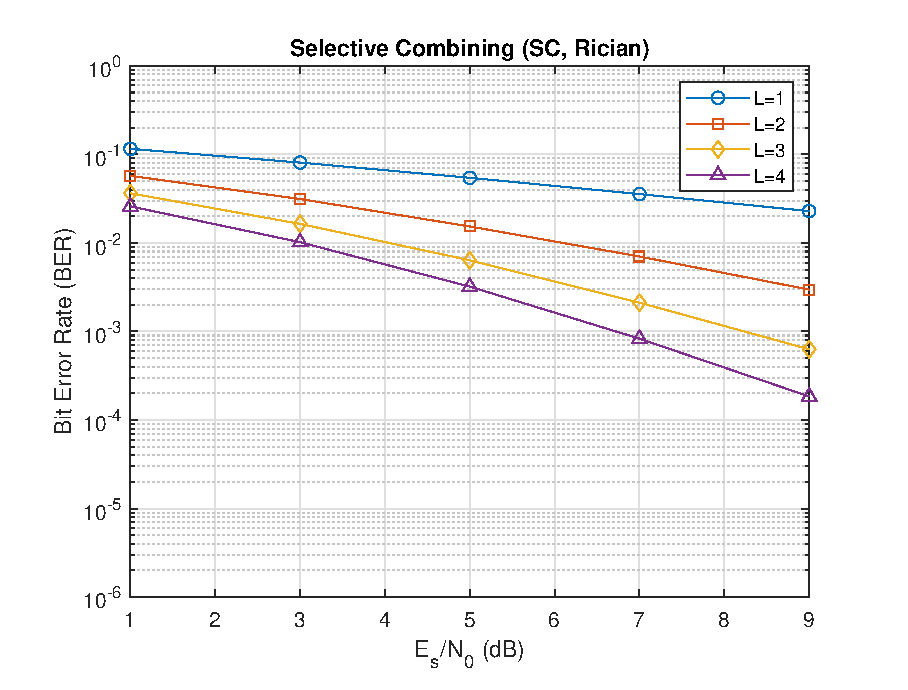
\includegraphics[scale = 0.85]{SC_rician.eps}
    \end{figure}
    \item[(b)] \textbf{Maximal Ratio Combinig (MRC)} \hfill \\
    \begin{figure}[H]
        \centering
        \includegraphics[scale = 0.85]{MRC_rician.eps}
    \end{figure}
    \item[(c)] \textbf{Equal Gain Combinig (MRC)} \hfill \\
    \begin{figure}[H]
        \centering
        \includegraphics[scale = 0.85]{EGC_rician.eps}
    \end{figure}
    \item[(d)] \textbf{Direct Combinig (MRC)} \hfill \\
    \begin{figure}[H]
        \centering
        \includegraphics[scale = 0.85]{DC_rician.eps}
    \end{figure}
\end{itemize}